% --------------------------------------------------------------
% This is all preamble stuff that you don't have to worry about.
% Head down to where it says "Start here"
% --------------------------------------------------------------
 
\documentclass[12pt]{article}
 
\usepackage[margin=1in]{geometry} 
\usepackage{bm} % bold in mathmode \bm
\usepackage{amsmath,amsthm,amssymb,mathtools}
\usepackage{dsfont} % for indicator function \mathds 1
\usepackage{tikz,pgf,pgfplots}
\usepackage{enumerate} 
\usepackage[multiple]{footmisc} % for an adjascent footnote
\usepackage{graphicx,float} % figures
\usepackage{framed} % surround a text with a box 

\newtheorem{definition}{Definition}
\let\olddefinition\definition
\renewcommand{\definition}{\olddefinition\normalfont}
\newtheorem{lemma}{Lemma}
\let\oldlemma\lemma
\renewcommand{\lemma}{\oldlemma\normalfont}
\newtheorem{proposition}{Proposition}
\let\oldproposition\proposition
\renewcommand{\proposition}{\oldproposition\normalfont}
\newtheorem{corollary}{Corollary}
\let\oldcorollary\corollary
\renewcommand{\corollary}{\oldcorollary\normalfont}
\newtheorem{theorem}{Theorem}
\let\oldtheorem\theorem
\renewcommand{\theorem}{\oldtheorem\normalfont}

%%% PLOTTING PARAMETERS
\tikzstyle{bag} = [text width=7em, text centered] %binomial tree node width
\tikzstyle{end} = []

\pgfplotsset{soldot/.style={color=black,only marks,mark=*},
             holdot/.style={color=black,fill=white,only marks,mark=*},
             compat=1.12}
%%%

%% set noindent by default and define indent to be the standard indent length
\newlength\tindent
\setlength{\tindent}{\parindent}
\setlength{\parindent}{0pt}
\renewcommand{\indent}{\hspace*{\tindent}}

\newcommand*{\vv}[1]{\vec{\mkern0mu#1}} % \vec command

%% DAVIDS MACRO KIT %%
\newcommand{\R}{\mathbb R}
\newcommand{\N}{\mathbb N}
\newcommand{\Z}{\mathbb Z}
\renewcommand{\P}{\mathbb P}
\newcommand{\Q}{\mathbb Q}
\newcommand{\E}{\mathbb E}
\newcommand{\var}{\mathrm{Var}}
\newcommand{\Var}{\mathrm{Var}}
\newcommand{\cov}{\mathrm{Cov}}
\newcommand{\Cov}{\mathrm{Cov}}
\newcommand{\indist}{\,{\buildrel \mathcal D \over \sim}\,}

\newcommand{\bigtau}{\text{{\large $\bm \tau$}}}


%%
\newcounter{mycounter}

\begin{document}
 
% --------------------------------------------------------------
%                         Start here
% --------------------------------------------------------------
 
\title{Mathematical \& Computational Finance I\\Lecture Notes}
\author{Generalizing American Derivative Securities}
\date{March 10 2016 \\ Last update: \today{}}
\maketitle

% SECTION: 
\section{General American Derivative Securities (con't)}

\indent In the last set of notes we had proven that the American algorithm generalizes to path-dependent American derivative securities. Furthermore, we had also shown that the stopping time
\begin{equation*}
	\tau^* = \min\{n:V_n = G_n\}
\end{equation*}

is the stopping time that maximizes the conditional expectation 
\begin{equation*}
	V_n = \max_{\tau \in \mathcal S_n} \tilde{\E}_n \left[ \mathds 1_{\{\tau \leq N\}} \frac{1}{(1 + r)^{\tau - n}} G_\tau \right]
\end{equation*}

From the Replication Theorem we had that
\begin{align*}
	V_n &= X_n \quad \text{and in particular,} \\
	X_n &\geq G_n
\end{align*}

\indent However, the Optimal Stopping/Exercise Theorem states that {\bf the long party should stop/exercise the first time $\bm{V_n = G_n}$.} It may be the case that these quantities will never be equal (e.g. a put that is always above the strike). In the case that $V_n \neq G_n~\forall\, n$ then we minimize over the empty set to find $\tau^* = \infty$ (i.e. never exercise). \\

\underline{Example:} {\em (Example from a past exam)} Consider a $N = 4$ period binomial model with $S_0 = 50, u = 1.2, d = 0.80, r = 0.1$.
\begin{enumerate}[(a)]
	\item Find the time-zero price of an American put with $K = 35$. \\
	
	We first build our stock tree	
	\begin{figure}[H]
	\centering
	\begin{tikzpicture}[sloped]
	  \node (a) at ( 0,0) [bag] {$50$};
	  \node (b) at ( 2,-1) [bag] {$40$};
	  \node (c) at ( 2,1) [bag] {$60$};
	  \node (d) at ( 4,-2) [bag] {$32$};
	  \node (e) at ( 4,0) [bag] {$48$};
	  \node (f) at ( 4,2) [bag] {$72$};
	  \node (g) at ( 6,-3) [bag] {$25.60$};
	  \node (h) at ( 6,-1) [bag] {$35.40$};
	  \node (i) at ( 6,1) [bag] {$57.60$};
	  \node (j) at ( 6,3) [bag] {$86.40$};
	  \node (l) at ( 8,-4) [bag] {$20.48$};
	  \node (m) at ( 8,-2) [bag] {$30.72$};
	  \node (n) at ( 8,0) [bag] {$46.08$};
	  \node (o) at ( 8,2) [bag] {$69.12$};
	  \node (p) at ( 8,4) [bag] {$103.68$};

	  \draw [->] (a) to node [below] {} (b);
	  \draw [->] (a) to node [above] {} (c);
	  \draw [->] (c) to node [below] {} (f);
	  \draw [->] (c) to node [above] {} (e);
	  \draw [->] (b) to node [below] {} (e);
 	  \draw [->] (b) to node [above] {} (d);
	  \draw [->] (d) to node [above] {} (g);
	  \draw [->] (d) to node [above] {} (h);
	  \draw [->] (e) to node [above] {} (h);
	  \draw [->] (e) to node [above] {} (i);
	  \draw [->] (f) to node [above] {} (i);
	  \draw [->] (f) to node [above] {} (j);
	  \draw [->] (g) to node [above] {} (l);
	  \draw [->] (g) to node [above] {} (m);
	  \draw [->] (h) to node [above] {} (m);
	  \draw [->] (h) to node [above] {} (n);
	  \draw [->] (i) to node [above] {} (n);
	  \draw [->] (i) to node [above] {} (o);
	  \draw [->] (j) to node [above] {} (o);
	  \draw [->] (j) to node [above] {} (p);
	\end{tikzpicture}
	\caption{Asset price tree $S_n$.}
	\end{figure}
	
	Then, with intrinsic value function $g(s) = (K - s) = 35 - s$ we have the $\max(0, g(S_n))$ process
	\begin{figure}[H]
	\centering
	\begin{tikzpicture}[sloped]
	  \node (a) at ( 0,0) [bag] {$0$};
	  \node (b) at ( 2,-1) [bag] {$0$};
	  \node (c) at ( 2,1) [bag] {$0$};
	  \node (d) at ( 4,-2) [bag] {$3$};
	  \node (e) at ( 4,0) [bag] {$0$};
	  \node (f) at ( 4,2) [bag] {$0$};
	  \node (g) at ( 6,-3) [bag] {$9.40$};
	  \node (h) at ( 6,-1) [bag] {$0$};
	  \node (i) at ( 6,1) [bag] {$0$};
	  \node (j) at ( 6,3) [bag] {$0$};
	  \node (l) at ( 8,-4) [bag] {$14.52$};
	  \node (m) at ( 8,-2) [bag] {$4.28$};
	  \node (n) at ( 8,0) [bag] {$0$};
	  \node (o) at ( 8,2) [bag] {$0$};
	  \node (p) at ( 8,4) [bag] {$0$};

	  \draw [->] (a) to node [below] {} (b);
	  \draw [->] (a) to node [above] {} (c);
	  \draw [->] (c) to node [below] {} (f);
	  \draw [->] (c) to node [above] {} (e);
	  \draw [->] (b) to node [below] {} (e);
 	  \draw [->] (b) to node [above] {} (d);
	  \draw [->] (d) to node [above] {} (g);
	  \draw [->] (d) to node [above] {} (h);
	  \draw [->] (e) to node [above] {} (h);
	  \draw [->] (e) to node [above] {} (i);
	  \draw [->] (f) to node [above] {} (i);
	  \draw [->] (f) to node [above] {} (j);
	  \draw [->] (g) to node [above] {} (l);
	  \draw [->] (g) to node [above] {} (m);
	  \draw [->] (h) to node [above] {} (m);
	  \draw [->] (h) to node [above] {} (n);
	  \draw [->] (i) to node [above] {} (n);
	  \draw [->] (i) to node [above] {} (o);
	  \draw [->] (j) to node [above] {} (o);
	  \draw [->] (j) to node [above] {} (p);
	\end{tikzpicture}
	\caption{The $\max(0, g(S_n))$ process.}
	\end{figure}
	
	and using our American pricing algorithm for the time $n$ price $V_n$
	\begin{equation*}
		V_n = \max \left\{ g(S_n), \frac{1}{1 + r}\Big[ \tilde{p}V_{n + 1}(H) + \tilde{q}V_{n + 1}(T) \Big] \right\} \quad n = N - 1,..., 1, 0
	\end{equation*}
	
	Now, with
	\begin{align*}
		\tilde{p} &= \frac{(1 + r) - d}{u - d} \\
		&= \frac{1.10 - 0.80}{1.20 - 0.80} \\
		&= 0.75
	\end{align*}
	
	we are able to easily find the process/tree for $V_n$
		\begin{figure}[H]
	\centering
	\begin{tikzpicture}[sloped]
	  \node (a) at ( 0,0) [bag] {$0.223473465$};
	  \node (b) at ( 2,-1) [bag] {$0.832550714$};
	  \node (c) at ( 2,1) [bag] {$0.050244177$};
	  \node (d) at ( 4,-2) [bag] {$3$};
	  \node (e) at ( 4,0) [bag] {$0.22107438$};
	  \node (f) at ( 4,2) [bag] {$0$};
	  \node (g) at ( 6,-3) [bag] {$9.40$};
	  \node (h) at ( 6,-1) [bag] {$0.97272727$};
	  \node (i) at ( 6,1) [bag] {$0$};
	  \node (j) at ( 6,3) [bag] {$0$};
	  \node (l) at ( 8,-4) [bag] {$14.52$};
	  \node (m) at ( 8,-2) [bag] {$4.28$};
	  \node (n) at ( 8,0) [bag] {$0$};
	  \node (o) at ( 8,2) [bag] {$0$};
	  \node (p) at ( 8,4) [bag] {$0$};

	  \draw [->] (a) to node [below] {} (b);
	  \draw [->] (a) to node [above] {} (c);
	  \draw [->] (c) to node [below] {} (f);
	  \draw [->] (c) to node [above] {} (e);
	  \draw [->] (b) to node [below] {} (e);
 	  \draw [->] (b) to node [above] {} (d);
	  \draw [->] (d) to node [above] {} (g);
	  \draw [->] (d) to node [above] {} (h);
	  \draw [->] (e) to node [above] {} (h);
	  \draw [->] (e) to node [above] {} (i);
	  \draw [->] (f) to node [above] {} (i);
	  \draw [->] (f) to node [above] {} (j);
	  \draw [->] (g) to node [above] {} (l);
	  \draw [->] (g) to node [above] {} (m);
	  \draw [->] (h) to node [above] {} (m);
	  \draw [->] (h) to node [above] {} (n);
	  \draw [->] (i) to node [above] {} (n);
	  \draw [->] (i) to node [above] {} (o);
	  \draw [->] (j) to node [above] {} (o);
	  \draw [->] (j) to node [above] {} (p);
	\end{tikzpicture}
	\caption{American derivative security price process $V_n$.}
	\end{figure}
	
	as desired. {\bf Note that if we wish to find the optimal stopping time we should look for the first time where $\bm{V_n = G_n}$.} We find this at $V_n = G_n = 3$ at $n = 2$.
	
	\item Give the replicating portfolio process at all nodes of the tree. \\
	
	With 
	\begin{align*}
		v_n(S_n(\omega_1 \cdots \omega_n)) &= V_n(\omega_1\cdots\omega_n) \\
		\delta_n(S_n(\omega_1\cdots\omega_n)) &= \Delta_n(\omega_1\cdots\omega_n) 
	\end{align*}
	
	we can easily find
	\begin{align*}
		\delta_0 &= \frac{v_1(60) - v_1(40)}{60 - 40} = \frac{ 0.05024417   0.832550714 }{ 20 } = -0.039115327 \\
		\delta_1(60) &= \frac{ v_2(72) - v_2(48) }{72 - 48} = \frac{ 0 - 0.22107438 }{24} = -0.009211433 \\
		\delta_1(40) &= \frac{ v_2(48) - v_2(32) }{48 - 32} = \frac{0.221074338 - 3}{16} = -0.173682851 \\
		\delta_2(72) &= \frac{ v_3(86.40) - v_3(57.60) }{ 86.40 - 57.60 } = 0 \\
		\delta_2(48) &= \frac{ v_3(57.60) - v_3(38.40) }{ 57.60 - 38.40 } = \frac{0 - 0.97272727 }{ 19.2 } = -0.050662879 \\ \\
		\delta_2(32) &= \frac{ v_3(38.40) - v_3(25.60) }{ 38.40 - 25.60 } = \frac{ 0.97272727 - 9.40 }{ 12.8 } = -0.658380682 \\
		\delta_3(86.40) &= \cdots \text{{\em apply magic}} \cdots = 0 \\
		\delta_3(57.60 &= \cdots \text{{\em apply magic}} \cdots = 0 \\
		\delta_3(38.40) &= \cdots \text{{\em apply magic}} \cdots  = -0.278645833 \\
		\delta_3(25.60) &= \cdots \text{{\em apply magic}} \cdots = -1
	\end{align*}
	
	as desired.
	
	\item What is the optimal exercise strategy for part (a)? \\
	
	\indent By our Optimal Exercise Theorem we have that, letting $\tau^*$ denote such an optimal stopping time, $\tau^*$ is the earliest time $V_n = G_n$. We can easily compare our $V_n$ tree with our intrinsic value tree $G_n$ to find $\tau^*(\bar{\omega})$, for $\bar{\omega}$ a sequence of coin tosses in $\Omega$,
	\begin{equation*}
		\tau^* =
		\begin{cases}
			2 & \text{if } \omega_1\omega_2 = TT \\
			4 & \text{if } \omega_1\omega_2\omega_3\omega_4 = THTT, HTTT \\
			\infty & \text{else}
		\end{cases}
	\end{equation*}
	
	\item Suppose now that $\omega_1\omega_2 = TT$. If the long party of the option {\bf does not} exercise the option at time $t = 2$ (i.e. suboptimal exercise) how much is the short party able to consume at $t = 2$ (i.e. find $C_2(TT)$). Furthermore, if $\omega_3 = T$ verify that the value of the short party's hedging portfolio at time $t = 3$ is the same value as the option (i.e. verify $X_3(TTT) = V_3(TTT)$). 
	
	Recall that we had found the consumption process $C_n(\omega_1\cdots\omega_n)$ to be
	\begin{equation*}
		C_n = V_n - \frac{1}{1 + r}\Big[\tilde{p}V_{n + 1}(H) + \tilde{q}V_3(T)\Big]
	\end{equation*}
	
	Therefore, with	$\omega_1\omega_2 = TT$ and $S_2(TT) = 32$ we have
	\begin{align*}
		c_2(32) &= v_2(32) - \frac{1}{1 + r}\Big[\tilde{p}v_3(38.40) + \tilde{q}V_3(25.60)\Big] \\
		&= 3 - \frac{1}{1.1}\Big[0.75 \cdot 0.97272727 + 0.25\cdot9.40\Big] \\
		&= 0.200413223
	\end{align*}
	
	That is, the short party may consume $0.200413223$ if the long counterparty does not exercise at $\omega_1\omega_2 = TT$. If the third coin toss $\omega_3 = T$ then by the wealth equation for American options we have, with $x_n(S_n(\omega_1\cdots\omega_n) = X_n(\omega_1\cdots\omega_n)$,
	\begin{align*}
		X_3(TTT) &= \Delta_2(TT)S_3(TTT) + (1 + r) \Big[ X_2(TT) - C_2(TT) + \Delta_2(TT)S_2(TT) \Big] \\
		\implies x_3(25.60) &= \delta_2(25.60)\cdot25.60 + 1.1\cdot\Big[ x_2(32) - c_2(32) - \delta_2(32)\cdot 32 \Big] \\
		&= -0.658380682\cdot25.60 + 1.1\Big[3 - 0.200413223 + 0.658380682\cdot 32 ] \\
		&= -16.854545455 + 1.1 \cdot 23.867768601 \\
		&= 9.4 \\
		&= v_3(25.60) \\
		&= V_3(TTT)
	\end{align*}
	
	as desired.	
\end{enumerate}

\section{American Call Options}

\indent We may have seen before (in some introductory finance course) that it is {\bf never optimal} to exercise early given an American call option written on a non-dividend paying stock. If we are able to prove this then we can price an American call just as we would price a vanilla European call, saving us plenty of time. \\

Let $g:[0,\infty)\to\R$ be a convex function\footnote{We should think of $g$ as analogous to our call payoff function.} with $g(0) = 0$. Since $g$ is convex, we have from Jensen's inequality
\begin{equation*}
	g(\lambda s_1 + (1 - \lambda)s_2) \leq \lambda g(s_1) + (1 - \lambda)g(s_2)
\end{equation*}

for all $s_1,s_2 \in [0,\infty)$ and $\lambda \in [0,1]$. In particular, our call option payoff function
\begin{equation*}
	g(s) = (s - K)^+
\end{equation*}

is a convex function, as illustrated below.


\begin{figure}[H]
\centering
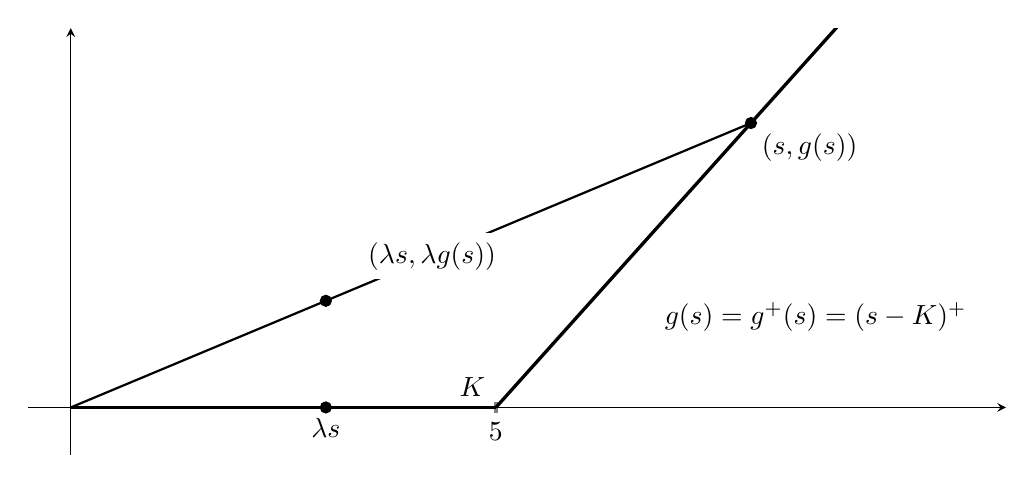
\begin{tikzpicture}
	\begin{axis}[axis lines=middle,
		width = 14cm,height=7cm,
 		xmin=-0.5,xmax=11,
 		ymin=-0.5,ymax=4,
		xtick=\empty,xticklabels=\empty,
		x tick style={very thick},
		ytick=\empty,yticklabels=\empty,
		extra x ticks={5}]
	\addplot[soldot] coordinates{(3,0)(8,3)(3,1.125)};
	\draw[black, very thick] (0,0) -- (5,0) node[above left ] {$K$};
	\draw[black, very thick] (5,0) -- (8,3) node[below right] {$(s, g(s))$};
	\draw[black, very thick] (8,3) -- (10,5) node[below right] {$(s, g(s))$};
	\draw[black, very thick] (0,0) -- (3,0) node[below] {$\lambda s$};
	\draw[black, thick] (0,0) -- (3,1.125);
	\draw[black, thick] (3,1.125) -- (8,3) node[near start,fill=white] {$(\lambda s, \lambda g(s))$};
	\end{axis}
	\node at (10,1.75) {$g(s) = g^+(s) = (s - K)^+$};
\end{tikzpicture}
\caption{Convex function $g$ with $g(0) = 0$.}
\end{figure}

\begin{theorem} Consider the $N$-period binomial asset pricing model with $0 < d < 1 + r  < u$ and\footnote{Notice that before we required $r > -1$ to avoid dividing by zero. We now restrict ourselves to $r \geq 0$ for the purposes of this proof.} $r \geq 0$. Consider an \underline{American} derivative security with convex payoff function $g(s)$ satisfying $g(0) = 0$. The value of this derivative security at time zero is, by definition,
\begin{equation*}
	V^A_0 = \max_{\tau \in \mathcal S_0} \tilde{\E}_0 \left[ \mathds 1_{\{\tau \leq N\}} \frac{1}{(1 + r)^\tau} g(S_\tau) \right]
\end{equation*}

and this value $V^A_0$ is the same value as the price of an equivalent \underline{European} derivative security with payoff $g(S_N)$ at time $N$ given by
\begin{equation*}
	V^E_0 = \tilde{\E} \left[ \frac{1}{(1 + r)^N} g(S_N) \right]
\end{equation*}

That is, $V^A_0 = V^E_0$.

\begin{proof} Define $g^+(s) := \max \{g(s), 0\}$. We have that that $g$ is a convex function. We will first show that $g^+$ must also be convex. By Jensen's inequality, for $\lambda \in [0,1]$ and $s_1, s_2 \in [0, \infty)$,
\begin{equation*}
	g(\lambda s_1 + (1 - \lambda)s_2) \leq \lambda g(s_1) + (1 - \lambda)g(s_2)
\end{equation*}

But by definition of $g^+(s)$ we have
\begin{align*}
	g^+((\lambda s_1 + (1 - \lambda)s_2) &= \max \Big\{0, g((\lambda s_1 + (1 - \lambda)s_2) \Big\} \\
	\implies 0 &\leq g^+(\lambda s_1 + (1 - \lambda)s_2) \\
	&\leq \lambda g^+(s_1) + (1 - \lambda)g^+(s_2)
\end{align*}

So
\begin{align*}
	g^+(\lambda s_1 + (1 - \lambda)s_2) &= \max \big\{0, g(\lambda s_1 + (1 - \lambda)s_2) \big\} \\
	&\leq \max \Big\{0, \lambda g(s_1) + (1 - \lambda)g(s_2) \Big\} \\
	&\leq \max \Big\{0, \lambda g^+(s_1) + (1 - \lambda)g^+(s_2) \Big\} \\
	&= \lambda g^+(s_1) + (1 - \lambda)g^+(s_2)
\end{align*}

So $g^+$ is indeed convex. Now, taking $s_1 = s$ and $s_2 = 0$ gives us
\begin{equation*}
	g^+(\lambda s) \leq \lambda g^+(s) \quad \forall\,s \geq 0,~\lambda\in[0,1]
\end{equation*}

\indent Under the risk-neutral measure $\tilde{\P}$ we have that the discounted asset price process $\left\{ \frac{S_n}{(1 + r)^n} \right\}^N_{n = 0}$ is a martingale. That is,
\begin{equation*}
	S_n = \tilde{\E}_n \left[ \frac{S_{n + 1}}{1 + r} \right]
\end{equation*}

and evaluating $g^+$ at $S_n$ we get
\begin{equation*}
	g^+(S_n) = g^+ \left( \tilde{\E}_n \left[ \frac{S_{n + 1}}{1 + r} \right] \right)
\end{equation*}

Since $g^+$ is convex we apply (conditional) Jensen's inequality\footnote{$\E_n[\psi(X)] \geq \psi(\E_n[X])$, for convex $\psi$.}
\begin{align*}
	g^+(S_n) &= g^+ \left( \tilde{\E}_n \left[ \frac{S_{n + 1}}{1 + r} \right] \right) \\
	&\leq \tilde{\E}_n \left[ g^+ \left( \frac{S_{n + 1}}{1 + r} \right) \right]
\end{align*}

We now let $\lambda = \frac{1}{1 + r} \in [0,1]$ (note that this substitution requires that $r \geq 0$) to find
\begin{align*}
	g^+(S_n) &\leq \tilde{\E}_n \left[ \frac{ g^+ \left( S_{n + 1} \right) }{1 + r} \right] \\
	\implies \frac{ g^+(S_n) }{(1 + r)^n} &\leq \tilde{\E}_n \left[ \frac{ g^+ \left( S_{n + 1} \right) }{(1 + r)^{n + 1}} \right]
\end{align*}

This informs us that the discounted max payoff process
\begin{equation*}
	\left\{  \frac{ g^+ \left( S_{n + 1} \right) }{(1 + r)^{n + 1}} \right\}^N_{n = 0}
\end{equation*}

satisfies the submartingale property with respect to the risk-neutral measure $\tilde{\P}$. Since this discounted process is a function of an adapted process we have that $\left\{  \frac{ g^+ \left( S_{n + 1} \right) }{(1 + r)^{n + 1}} \right\}^N_{n = 0}$ is a $\tilde{\P}$-submartingale. Applying the Optional Sampling Theorem\footnote{Let $\tau$ be a stopping time. If $X_n$ is a supermartingale then $\E[X_{n\land\tau}] \geq \E[X_n]$. If $X_n$ is a submartingale then $\E[X_{n\land\tau}] \leq \E[X_n]$. If $X_n$ is a martingale then $\E[X_{n\land\tau}] = \E[X_n]$. This matches with our intuition of super and submartingales.} we have
\begin{align*}
	\frac{ g^+(S_0) }{(1 + r)^0} &\leq \tilde{\E}_0 \left[ \frac{ g^+ \left( S_{N\land\tau} \right) }{(1 + r)^{N\land\tau}} \right] \\
	&\leq \tilde{\E}_0 \left[ \frac{ g^+ \left( S_N \right) }{(1 + r)^N} \right] \quad \text{(by the Optional Sampling Theorem)} \\
	&= V^E_0 \quad \forall\,\tau \in \mathcal S_0 
\end{align*}

If $\tau \leq N$ we find
\begin{align*}
	\mathds 1_{\{\tau\leq N\}} \frac{g(S_\tau)}{(1 + r)^\tau} &= \frac{ g(S_{N\land\tau}) }{(1 + r)^{N\land\tau}} \\
	&\leq \frac{ g^+(S_{N\land\tau}) }{(1 + r)^{N\land\tau}} \quad \text{(since $g^+$ is the max process)}
\end{align*}

and if $\tau = \infty$ then
\begin{align*}
	\mathds 1_{\{\tau \leq N\}} \frac{g(S_\tau)}{(1 + r)^\tau} &= 0\\
	&\leq  \frac{ g^+(S_{N\land\tau}) }{(1 + r)^{N\land\tau}}
\end{align*}

Hence, since both cases for $\tau$ are identical,
\begin{align*}
	\tilde{\E}_0 \left[ \mathds 1_{\{\tau \leq N\}} \frac{1}{(1 + r)^\tau} g(S_\tau) \right] &\leq \tilde{\E}_0 \left[ \mathds 1_{\{\tau \leq N\}} \frac{1}{(1 + r)^{N\land\tau}} g^+(S_{N\land\tau}) \right] \\
	&\leq V^E_0 \quad \text{(from the previous step above)}
\end{align*}

\indent Since this inequality holds for arbitrary $\tau\in\mathcal S_0$ we have from the American risk-neutral pricing formula, considering the maximizing $\tau$,
\begin{equation*}
	V^A_0 = \max_{\tau\in\mathcal S_0} \tilde{\E}_0 \left[ \mathds 1_{\{\tau \leq N\}} \frac{1}{(1 + r)^{\tau}} g^+(S_\tau) \right] \leq V^E_0
\end{equation*}

We should now show that $V^A_0 \geq V^E_0$. Perhaps this intuitive\footnote{Frankly I'm not fully convinced yet by the more formal argument we're about to use...} since an American option adds an additional feature onto a vanilla European option. More formally, we may say that since $\tau = \tau(\omega_1\cdots\omega_N) = N$ for all sequences $\omega_1\cdots\omega_N \in \Omega$ is a valid stopping time in $\mathcal S_0$ we have that
\begin{equation*}
	V^A_0 \geq V^E_0
\end{equation*}

Therefore, by these two results we may conclude that
\begin{equation*}
	V^E_0 = V^A_0
\end{equation*}

as desired.
\end{proof}
\end{theorem}

\underline{Example:} {\em (Exercise 4.2)} Consider our typical binomial model with $N = 2, S_0 = 4, u = 2, d = \frac{1}{2}$, and $r = \frac{1}{4}$. We found that the time-zero price of an American put option with strike $K = 5$ was $V_0 = 1.36$. Consider now an agent borrowing 1.36 at time zero to purchase the put option. Explain how the agent may generate sufficient funds to repay the loan with $r = \frac{1}{4}$ by trading in the underlying stock $S$ and riskless money market accounts, as well as optimally exercising the put. \\

\indent In this particular example we were given stopping times (I believe that these were also optimal stopping times)
\begin{equation*}
	\tau(HH) = \infty,~\tau(HT) = 2,~\tau(TH) = \tau(TT) = 1
\end{equation*}

We can show that the trading strategy $\Delta_n$ for the long position is\footnote{This is something worthy of proof... I'm not sure that we actually prove this for the long position.}
\begin{equation*}
	\Delta_n(\omega_1\cdots\omega_n) = - \frac{ V_{n + 1}(\omega_1\cdots\omega_n H) - V_{n + 1}(\omega_1\cdots\omega_n T) }{ S_{n + 1}(\omega_1\cdots\omega_n H) - S_{n + 1}(\omega_1\cdots\omega_n T) }
\end{equation*}

\indent If we have $X_0 = 0$ initial wealth we may find the value of the long party's portfolio at time $t = n + 1$ by
\begin{equation*}
	X_{n + 1} = \Delta_n S_{n + 1} + \mathds 1_{\{ \tau = n + 1\}}(K - S_{n + 1}) + (1 + r)[X_n - \Delta_nS_n]
\end{equation*}

where $\mathds 1_{\{ \tau = n + 1\}}(K - S_{n + 1})$ is the payoff if the option is exercised optimally. Now, at time $t = 0$ we have (using our previous computations for $V_n(\bar{\omega})$)

\begin{equation*}
	\Delta_0 = -\frac{ V_1(H) - V_1(T) }{ S_1(H) - S_1(T) } = - \frac{ \frac{2}{5} - 3 }{ 8 - 2 } = \frac{13}{30}
\end{equation*}

If $\omega_1 = T$ we find
\begin{align*}
	X_1(T) &= \Delta_0S_1(T) + \mathds 1_{\{ \tau(T) = 1\}}(K - S_1(T)) + (1 + r)[X_0 - \Delta_0S_0] \\
	&= \frac{13}{30}\cdot 2 + 1 \cdot (5 - 2) + \frac{5}{4}\left[ 0 - \frac{13}{30}\cdot 4\right] \\
	&= \frac{26}{30} + 3 - \frac{260}{120} \\
	&= \frac{26}{30} + \frac{90}{30} - \frac{65}{30} \\
	&= \frac{26 + 90 - 65}{30} \\
	&= \frac{51}{30} = 1.70
\end{align*}

and the outstanding balance of the loan taking by the long party to purchase the option is
\begin{align*}
	(1 + r)V_0 &= \frac{5}{4}\cdot1.36 \\
	&= 1.70
\end{align*}

\indent Therefore, the long party is able to fully repay the loan by selling the portfolio with no further action necessary since we have exercised our option. If $\omega_1 = H$ we find
\begin{align*}
	X_1(H) &= \Delta_0S_1(H) + \mathds 1_{\{ \tau(H) = 1\}}(K - S_1(H)) + (1 + r)[X_0 - \Delta_0S_0] \\
	&= \frac{13}{30} \cdot 8 + 0 + \frac{5}{4}\left[ 0 - \frac{13}{30}\cdot 4 \right] \\
	&= \frac{104}{30} - {260}{120} \\
	&= \frac{104}{30} - \frac{65}{30} \\
	&= \frac{104 - 65}{30} \\
	&= \frac{39}{30} = 1.30
\end{align*}

since we did not exercise the option we continue by readjusting the portfolio with
\begin{equation*}
	\Delta_1(H) = -\frac{ V_2(HH) - V_2(HT) }{ S_2(HH) - S_2(HT) } = - \frac{0 - 1}{16 - 4} = \frac{1}{12}
\end{equation*}

Now, if $\omega_2 = h$ we have portfolio value
\begin{align*}
	X_2(HH) &= \Delta_1(H)S_2(HH) + \mathds 1_{\{ \tau(HH) = 2\}}(K - S_2(HH)) + (1 + r)[X_1(H) - \Delta_1(H)S_1(H)] \\
	&= \frac{1}{12}\cdot 16 + 0 + \frac{5}{4}\left[ 1.30 - \frac{1}{12}\cdot 8 \right] \\
	&= 2.125
\end{align*}

with the balance of the loan $(1 + r)^2V_0 = (1.25)^2\cdot 1.36 = 2.125$. Therefore, if $\omega_1 = H, \omega_2 = H$ the long party is able to repay the loan by liquidating the portfolio with no further action necessary (since the option as expired). Finally, if $\omega_2 = T$ we find
\begin{align*}
	X_2(HT) &= \Delta_1(H)S_2(HT) + \mathds 1_{\{ \tau(HT) = 2\}}(K - S_2(HT)) + (1 + r)[X_1(H) - \Delta_1(H)S_1(H)] \\
	&= \frac{1}{12}\cdot 4 + 1\cdot (5 - 4) + \frac{5}{4}\left[ 1.30 - \frac{1}{12}\cdot 8 \right] \\
	&= 2.125
\end{align*}

\indent Once again we find that the long party is able to repay the loan. Therefore, in all scenarios, the long party is able to repay the loan used to purchase the American put assuming optimal exercise. \\

\underline{Example:} {(\em Exercise 4.3)} In the $N = 3$ period model with $S_0 = 4, u = 2, d = \frac{1}{2}$, and $r = \frac{1}{4}$ we found risk-neutral probabilities to be $\tilde{p} = \tilde{q} = \frac{1}{2}$. Find the time-zero price and optimal exercise strategy (optimal stopping times) for the path-dependent American derivative security whose intrinsic value at each step $n = 0,1,2,3$ is given by
\begin{equation*}
	g(S_0,...,S_n) = \left(4 - \frac{1}{n + 1}\sum^n_{j = 0} S_j \right)^+
\end{equation*} 

We construct the average process $\bar{X}_n = \frac{1}{n + 1}\sum^n_{j = 0}S_j$ with the tree
\begin{figure}[H]
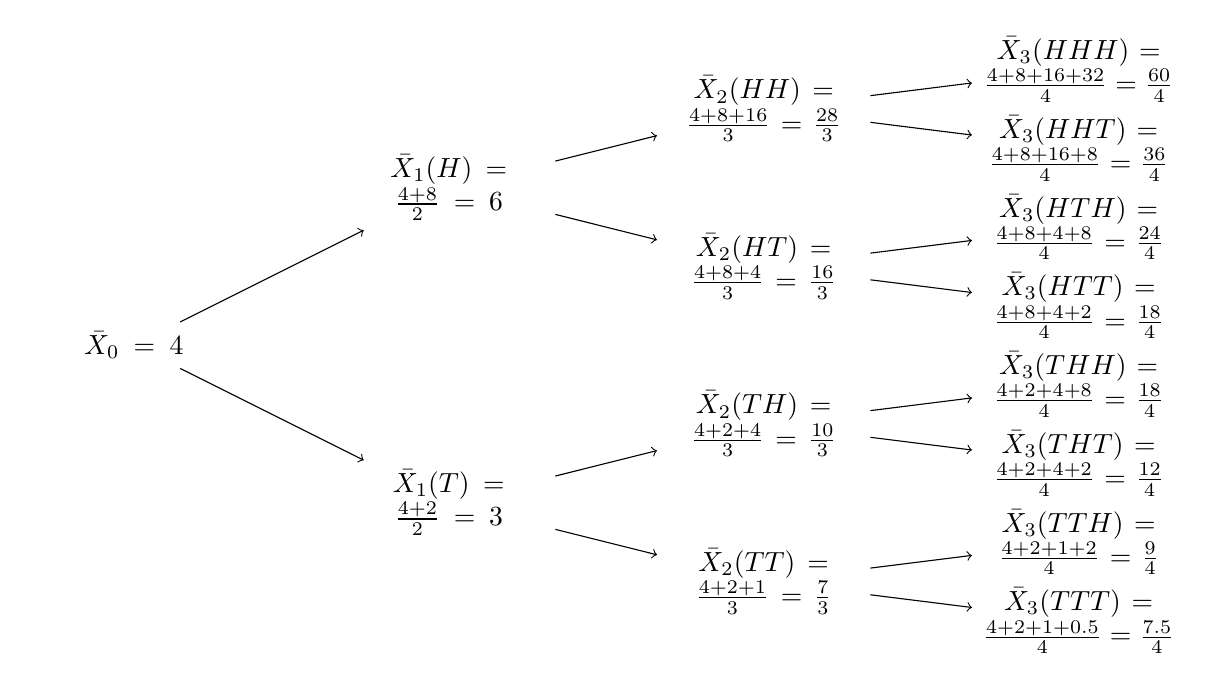
\begin{tikzpicture}[sloped]
  \node (a) at ( 0,0) [bag] {$\bar{X}_0 = 4$};
  \node (b) at ( 4,-2) [bag] {$\bar{X}_1(T) = \frac{4 + 2}{2} = 3$};
  \node (c) at ( 4,2) [bag] {$\bar{X}_1(H) = \frac{4 + 8}{2} = 6$};
  \node (d) at ( 8,-3) [bag] {$\bar{X}_2(TT) = \frac{4 + 2 + 1}{3} = \frac{7}{3}$};
  \node (e) at ( 8,-1) [bag] {$\bar{X}_2(TH) = \frac{4 + 2 + 4}{3} = \frac{10}{3}$};
  \node (f) at ( 8,1) [bag] {$\bar{X}_2(HT) = \frac{4 + 8 + 4}{3} = \frac{16}{3}$};
  \node (g) at ( 8,3) [bag] {$\bar{X}_2(HH) = \frac{4 + 8 + 16}{3} = \frac{28}{3}$};
  \node (h) at ( 12,-3.5) [bag] {$\bar{X}_3(TTT) = \frac{4 + 2 + 1 + 0.5}{4} = \frac{7.5}{4}$};
  \node (i) at ( 12,-2.5) [bag] {$\bar{X}_3(TTH) = \frac{4 + 2 + 1 + 2}{4} = \frac{9}{4}$};
  \node (j) at ( 12,-1.5) [bag] {$\bar{X}_3(THT) = \frac{4 + 2 + 4 + 2}{4} = \frac{12}{4}$};
  \node (k) at ( 12,-0.5) [bag] {$\bar{X}_3(THH) = \frac{4 + 2 + 4 + 8}{4} = \frac{18}{4}$};
  \node (l) at ( 12,0.5) [bag] {$\bar{X}_3(HTT) = \frac{4 + 8 + 4 + 2}{4} = \frac{18}{4}$};
  \node (m) at ( 12,1.5) [bag] {$\bar{X}_3(HTH) = \frac{4 + 8 + 4 + 8}{4} = \frac{24}{4}$};
  \node (n) at ( 12,2.5) [bag] {$\bar{X}_3(HHT) = \frac{4 + 8 + 16 + 8}{4} = \frac{36}{4}$};
  \node (o) at ( 12,3.5) [bag] {$\bar{X}_3(HHH) = \frac{4 + 8 + 16 + 32}{4} = \frac{60}{4}$};
  \draw [->] (a) to node [below] {} (b);
  \draw [->] (a) to node [above] {} (c);
  \draw [->] (b) to node [below] {} (d);
  \draw [->] (b) to node [above] {} (e);
  \draw [->] (c) to node [below] {} (f);
  \draw [->] (c) to node [above] {} (g);
  \draw [->] (d) to node [below] {} (h);
  \draw [->] (d) to node [above] {} (i);
  \draw [->] (e) to node [below] {} (j);
  \draw [->] (e) to node [above] {} (k);
  \draw [->] (f) to node [below] {} (l);
  \draw [->] (f) to node [above] {} (m);
  \draw [->] (g) to node [above] {} (n);  
  \draw [->] (g) to node [above] {} (o);  
\end{tikzpicture}
\caption{$\bar{X}_n$ process tree.}
\end{figure}

We can find the (max) intrinsic value tree given by $g_n(\bar{X}_n) = \max\{0, 4 - \bar{X}_n\}$
\begin{figure}[H]
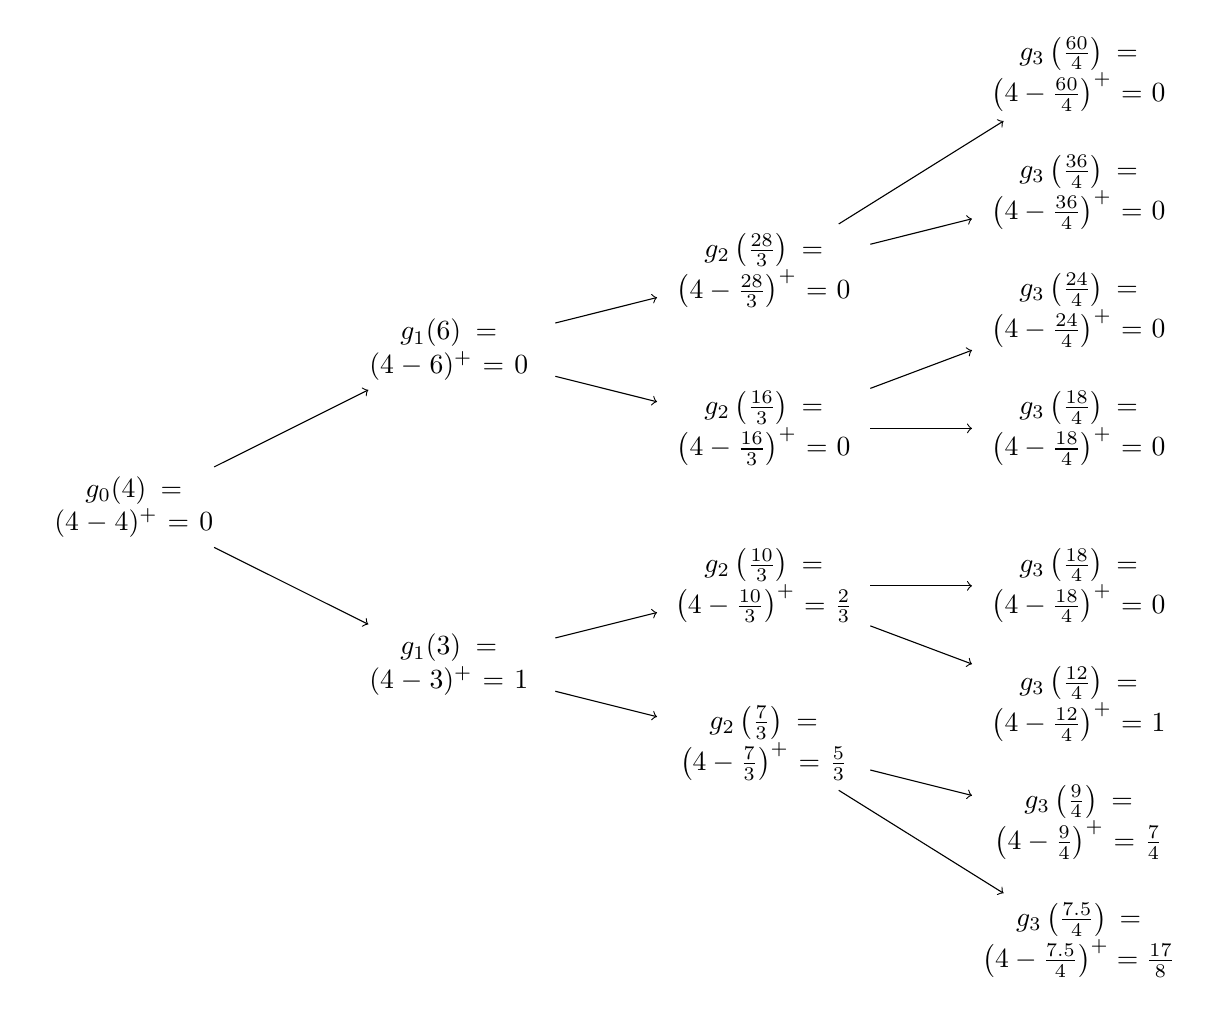
\begin{tikzpicture}[sloped]
  \node (a) at ( 0,0) [bag] {$g_0(4) = (4 - 4)^+ = 0$};
  \node (b) at ( 4,-2) [bag] {$g_1(3) = (4 - 3)^+ = 1$};
  \node (c) at ( 4,2) [bag] {$g_1(6) = (4 - 6)^+ = 0$};
  \node (d) at ( 8,-3) [bag] {$g_2\left( \frac{7}{3} \right) = \left(4 - \frac{7}{3}\right)^+ = \frac{5}{3}$};
  \node (e) at ( 8,-1) [bag] {$g_2\left( \frac{10}{3} \right) = \left(4 - \frac{10}{3}\right)^+ = \frac{2}{3}$};
  \node (f) at ( 8,1) [bag] {$g_2\left( \frac{16}{3} \right) = \left(4 - \frac{16}{3}\right)^+ = 0$};
  \node (g) at ( 8,3) [bag] {$g_2\left( \frac{28}{3} \right) = \left(4 - \frac{28}{3}\right)^+ = 0$};
  \node (h) at ( 12,-5.5) [bag] {$g_3\left( \frac{7.5}{4} \right) = \left( 4 - \frac{7.5}{4} \right)^+ = \frac{17}{8} $};
  \node (i) at ( 12,-4) [bag] {$g_3\left( \frac{9}{4} \right) = \left( 4 - \frac{9}{4} \right)^+ = \frac{7}{4}$};
  \node (j) at ( 12,-2.5) [bag] {$g_3\left( \frac{12}{4} \right) = \left( 4 - \frac{12}{4} \right)^+ = 1$};
  \node (k) at ( 12,-1) [bag] {$g_3\left( \frac{18}{4} \right) = \left( 4 - \frac{18}{4} \right)^+ = 0$};
  \node (l) at ( 12,1) [bag] {$g_3\left( \frac{18}{4} \right) = \left( 4 - \frac{18}{4} \right)^+ = 0$};
  \node (m) at ( 12,2.5) [bag] {$g_3\left( \frac{24}{4} \right) = \left( 4 - \frac{24}{4} \right)^+ = 0$};
  \node (n) at ( 12,4) [bag] {$g_3\left( \frac{36}{4} \right) = \left( 4 - \frac{36}{4} \right)^+ = 0$};
  \node (o) at ( 12,5.5) [bag] {$g_3\left( \frac{60}{4} \right) = \left( 4 - \frac{60}{4} \right)^+ = 0$};
  \draw [->] (a) to node [below] {} (b);
  \draw [->] (a) to node [above] {} (c);
  \draw [->] (b) to node [below] {} (d);
  \draw [->] (b) to node [above] {} (e);
  \draw [->] (c) to node [below] {} (f);
  \draw [->] (c) to node [above] {} (g);
  \draw [->] (d) to node [below] {} (h);
  \draw [->] (d) to node [above] {} (i);
  \draw [->] (e) to node [below] {} (j);
  \draw [->] (e) to node [above] {} (k);
  \draw [->] (f) to node [below] {} (l);
  \draw [->] (f) to node [above] {} (m);
  \draw [->] (g) to node [above] {} (n);  
  \draw [->] (g) to node [above] {} (o);  
\end{tikzpicture}
\caption{The (max) intrinsic value tree $g_n(\bar{X}_n) = \max\{0, 4 - \bar{X}_n\}$.}
\end{figure}

\indent Using the recursive American pricing algorithm we are able to compute the time $n$ value of the option $V_n(\omega_1\cdots\omega_n)$. Note that if $\omega_1 = H$ then regardless of the path the option takes the subsequent value $V_n(H\omega_2\omega_3) = 0$. Therefore, the optimal strategy for this upper branch is
\begin{equation*}
	\tau(\omega_1\omega_2\omega_3) = \infty \quad \text{if } \omega_1 = H \forall\,\omega_2\omega_3
\end{equation*}

Now, focusing n the lower branch we find the terminal values
\begin{align*}
	V_3(THH) &= \max \{ 0, g_3(\bar{X}_3(THH))\} = 0 \\
	V_3(THT) &= \max \{ 0, g_3(\bar{X}_3(THH))\} = 1 \\
	V_3(TTH) &= \max \{ 0, g_3(\bar{X}_3(TTH))\} = \frac{7}{4} \\
	V_3(TTT) &= \max \{ 0, g_3(\bar{X}_3(TTT))\} = \frac{17}{8}
\end{align*}

Using the recursive algorithm we compute the time $t = 2$ value
\begin{align*}
	V_2(TH) &= \max \left\{ g_2(\bar{X}_2(TH)), \frac{1}{1 + r}\left[ \tilde{p} V_3(THH) + \tilde{q}V_3(THT)\right] \right\} \\
	&= \max \left\{ \frac{2}{3}, \frac{4}{5}\cdot\frac{1}{2}\left[ 0 + 1 \right] \right\} \\
	&= \max \left\{ \frac{2}{3}, \frac{2}{5} \right\} \\
	&= \frac{2}{3} \quad \text{(early exercise)} \\
	V_2(TT) &= \max \left\{ g_2(\bar{X}_2(TT)), \frac{1}{1 + r}\left[ \tilde{p} V_3(THH) + \tilde{q}V_3(TTT)\right] \right\} \\
	&= \max \left\{ \frac{5}{3}, \frac{4}{5}\cdot\frac{1}{2}\left[ \frac{7}{4} + \frac{17}{8} \right] \right\} \\ 
	&= \max \left\{ \frac{5}{3}, \frac{31}{20} \right\} \\
	&= \frac{5}{3} \quad \text{(early exercise)}
\end{align*}

and at time $t = 1$ we find
\begin{align*}
	V_1(T) &= \max \left\{ g_1(\bar{X}_1(T)), \frac{1}{1 + r}\left[ \tilde{p} V_2(TH) + \tilde{q}V_2(TT)\right] \right\} \\
	&= \max \left\{1, \frac{4}{5}\cdot\frac{1}{2}\left[ \frac{2}{3} + \frac{5}{3} \right] \right\} \\
	&= \max \left\{ 1, \frac{14}{15} \right\} \\
	&= 1 \quad \text{(early exercise)}
\end{align*}

Finally, at time $t = 0$ we get
\begin{align*}
	V_0 &= \max \left\{ g_0(\bar{X}_0), \frac{1}{1 + r}\left[ \tilde{p} V_1(H) + \tilde{q}V_1(T)\right] \right\} \\ 
	&= \max \left\{ 0, \frac{4}{5}\cdot\frac{1}{2}\left[ 0 + 1 \right] \right\} \\
	&= \max \left\{0, \frac{2}{5} \right\} \\
	&= \frac{2}{5}
\end{align*}

\indent By the Optimal Exercise Theorem we have the first time $V_n = G_n$ along the path $T\omega_2\omega_3$ is the first node $\omega_1 = T$. Therefore
\begin{equation*}
	\tau(\omega_1\omega_2\omega_3) = 1 \quad \text{if } \omega_1 = T \forall\,\omega_2\omega_3
\end{equation*}

Therefore, we have a stopping time for all possible paths $\omega_1\omega_2\omega_3$
\begin{equation*}
	\tau(\omega_1\omega_2\omega_3) = 
	\begin{cases}
		\infty & \text{if } \omega_1 = H \\
		1 & \text{if } \omega_2 = T
	\end{cases}, 
	\quad \forall\,\omega_2\omega_3
\end{equation*}

as desired. \\

\underline{Example:} {\em (Exercise 4.5)} Recall that from the Optimal Exercise Theorem that the maximum 
\begin{equation*}
	V_0 = \max_{\tau \in \mathcal S_0} \tilde{\E} \left[ \mathds 1_{\tau \leq N} \frac{1}{(1 + r)^\tau} G_\tau \right]
\end{equation*}

is computed over all possible stopping times in $\mathcal S_0$. For the same example as was done in Exercise 4.2 (above), list all stopping times in $\mathcal S_0$ (there are 26 of them), and from among them, list the stopping times that never exercise when the option is out of the money (there are 11). For each stopping time $\tau$ in the latter set compute
\begin{equation*}
	\tilde{\E} \left[ \mathds 1_{\{\tau \leq 2\}} \left(\frac{4}{5}\right)^\tau G_\tau \right]
\end{equation*}

Verify that the largest value for this expectation corresponds to the stopping time $\tau$ such that
\begin{equation*}
	\tau(HH) = \infty,~\tau(HT) = 2,~\tau(TH) = \tau(TT) = 1
\end{equation*}

found to yield $V_0  = 1.36$. \\

From this problem we had the intrinsic value process
\begin{figure}[H]
\centering
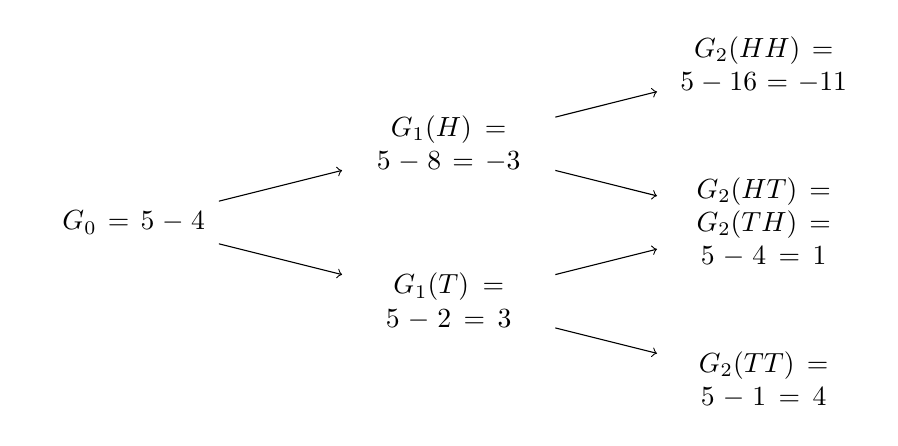
\begin{tikzpicture}[sloped]
  \node (a) at ( 0,0) [bag] {$G_0 = 5 - 4$};
  \node (b) at ( 4,-1) [bag] {$G_1(T) = 5 - 2 = 3$};
  \node (c) at ( 4,1) [bag] {$G_1(H) = 5 - 8 = -3$};
  \node (d) at ( 8,-2) [bag] {$G_2(TT) = 5 - 1 = 4$};
  \node (e) at ( 8,0) [bag] {$G_2(HT) = G_2(TH) = 5 - 4 = 1$};
  \node (f) at ( 8,2) [bag] {$G_2(HH) = 5 - 16 = -11$};
  \draw [->] (a) to node [below] {} (b);
  \draw [->] (a) to node [above] {} (c);
  \draw [->] (c) to node [below] {} (f);
  \draw [->] (c) to node [above] {} (e);
  \draw [->] (b) to node [below] {} (e);
  \draw [->] (b) to node [above] {} (d);
\end{tikzpicture}
\caption{Intrinsic value process $G_n$.}
\end{figure}

Recall that from the definition of a stopping time we require $\tau$ to satisfy
\begin{enumerate}[(i)]
	\item $\tau \in \{0,1,2\}\cup\{\infty\}$.
	\item If $\tau(\omega_1\omega_2) = n \implies \tau(\omega_1\omega'_2) = n,\quad \forall\,\omega'_2$.
\end{enumerate}

\indent In we consider just a few examples we find that for this particular option the contract would be exercised out of the money of $\tau(HH) = 2$, $\tau(HH) = 1$, or $\tau(HT) = 1$. We can enumerate the full list of stopping times and indicate if they result in an exercise out of the money
\begin{figure}[H]
\centering
\begin{tabular}{l|lllll}
	& $\tau(HH)$ & $\tau(HT)$ & $\tau(TH)$ & $\tau(TT)$ & Exer. OTM? \\
	\hline
	1 & 0 & 0 & 0 & 0 & No \\
	2 & 1 & 1 & 1 & 1 & Yes \\
	3 & 1 & 1 & 2 & 2 & Yes \\
	4 & 1 & 1 & $\infty$ & $\infty$ & Yes \\
	5 & 1 & 1 & 2 & $\infty$ & Yes \\
	6 & 1 & 1 & $\infty$ & 2 & Yes \\
	7 & 2 & 2 & 1 & 1 & Yes \\
	8 & 2 & 2 & 2 & 2 & Yes \\
	9 & 2 & 2 & $\infty$ & $\infty$ & Yes \\
	10 & 2 & 2 & $\infty$ & 2 & Yes \\
	11 & 2 & 2 & 2 & $\infty$ & Yes \\
	12 & $\infty$ & $\infty$ & 1 & 1 & No \\
	13 & $\infty$ & $\infty$ & 2 & 2 & No \\
	14 & $\infty$ & $\infty$ & $\infty$ & $\infty$ & No \\
	15 & $\infty$ & $\infty$ & 2 & $\infty$ & No \\
	16 & $\infty$ & $\infty$ & $\infty$ & 2 & No \\
	17 & $\infty$ & 2 & 1 & 1 & No \\
	18 & 2 & $\infty$ & 1 & 1 & Yes \\
	19 & $\infty$ & 2 & 2 & 2 & No \\
	20 & 2 & $\infty$ & 2 & 2 & Yes \\
	21 & 2 & $\infty$ & 2 & $\infty$ & Yes \\
	22 & $\infty$ & 2 & 2 & $\infty$ & No \\
	23 & 2 & $\infty$ & $\infty$ & 2 & Yes \\
	24 & $\infty$ & 2 & $\infty$ & 2 & No \\
	25 & $\infty$ & 2 & $\infty$ & $\infty$ & No \\
	26 & 2 & $\infty$ & $\infty$ & $\infty$ & Yes \\	
\end{tabular}
\end{figure}

Note that we we have 11 stopping times that do not lead to an exercise out of the money. Since we may ignore stopping times leading to OTM exercise, we may compute
\begin{equation*}
	X(\omega) = \mathds 1_{\{\tau \leq 2\}}(\omega) \frac{1}{(1 + r)^{\tau(\omega)}} G(\tau(\omega))
\end{equation*}

for stopping times with exercise in the money, and
\begin{equation*}
	\tilde{\E} \left[ \mathds 1_{\{\tau \leq 2\}} \frac{1}{(1 + r)^{\tau}} G(\tau) \right] = \sum_{\omega\in\Omega} \mathds 1_{\{\tau \leq 2\}}(\omega) \frac{1}{(1 + r)^{\tau(\omega)}} G(\tau(\omega)) \tilde{\P}(\omega)
\end{equation*}

We have $r = \frac{1}{4}$ and since all coin tosses are independent we have $\tilde{\P}(\omega) = \frac{1}{4}$. We are able to construct the following table for all ITM exercises
\begin{figure}[H]
\centering
\begin{tabular}{l|llllllll|l}
	& $\tau(HH)$ & $\tau(HT)$ & $\tau(TH)$ & $\tau(TT)$ & $X(HH)$ & $X(HT)$ & $X(TH)$ & $X(TT)$ & $\tilde{\E}[X]$ \\
	\hline
	1 & 0 & 0 & 0 & 0 & & 1 & 1 & 1 & 1 \\
	12 & $\infty$ & $\infty$ & 1 & 1 & 0 & 0 & 2.40 & 2.40 & 1.20 \\
	13 & $\infty$ & $\infty$ & 2 & 2 & 0 & 0 & 0.64 & 2.56 & 0.80 \\
	14 & $\infty$ & $\infty$ & $\infty$ & $\infty$ & 0 & 0 & 0 & 0 & 0 \\
	15 & $\infty$ & $\infty$ & 2 & $\infty$ & 0 & 0 & 0.64 & 0 & 0.16 \\
	16 & $\infty$ & $\infty$ & $\infty$ & 2 & 0 & 0 & 0 & 2.56 & 0.64 \\
	17 & $\infty$ & 2 & 1 & 1 & 0 & 0.64 & 2.40 & 2.40 & $\bm{1.36}$ \\
	19 & $\infty$ & 2 & 2 & 2 & 0 & 0.64 & 0.64 & 2.56 & 0.96 \\
	22 & $\infty$ & 2 & 2 & $\infty$ & 0 & 0.64 & 0.64 & 0 & 0.32 \\
	24 & $\infty$ & 2 & $\infty$ & 2 & 0 & 0.64 & 0 & 2.56 & 0.80 \\
	25 & $\infty$ & 2 & $\infty$ & $\infty$ & 0 & 0.64 & 0 & 0 & 0.16 \\
\end{tabular}
\end{figure}

Then, maximizing over the set of all stopping times we find
\begin{equation*}
	\max_{\tau \in \mathcal S_0} \tilde{\E} \left[ \mathds 1_{\{\tilde \leq 2\}} \frac{1}{(1 + r)^\tau} G(\tau) \right] = 1.36
\end{equation*}

which agrees with our previous calculations.











\end{document}
